\chapter{Creating a Sketch}

The most basic operation in any sketch-based modeling system is, of course, obtaining a sketch from the user.
The key characteristic of a sketch-capable input device is that it allows freehand input.
While a mouse is capable of this form of input, devices that more closely mimic the feel of freehand drawing using a pen, such as a digitizing tablet, are better for users to maximize their ability to draw.
Devices that are both an input device and a display are particularly suited to this, because it most closely mimics traditional artist creation methods by allowing direct interaction with the sketch space, as opposed to tablets where the space between the input device and the display surface is relative.

\begin{figure}
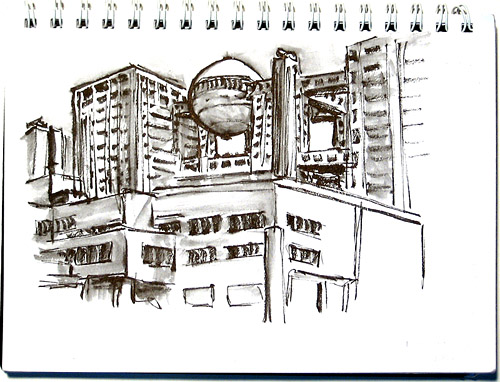
\includegraphics[width=0.7\textwidth]{fujitv}
\caption{An example of a sketch}
\end{figure}

Pencil and paper is a rich communication method. 
Artists convey information not only with the shape of the completed objects in the sketch, but also through more subtle methods such as pressure and stroke style.
Small details can relay information about the object, such as important details; heavier lines or many small strokes usually show more focus was put in a particular area.

\section{Representation of a Sketch}

At the bare minimum, an input device should provide positional information in some two dimensional coordinate system, usually one based on the interaction window.
For sketch input, the representation must at least approximate continuous movement.
Sampling rates vary from one device to the next.
The samples themselves may also be spaced irregularly, with sample points closer as users draw slowly or carefully, or father apart if the user draws quickly.

\begin{figure}
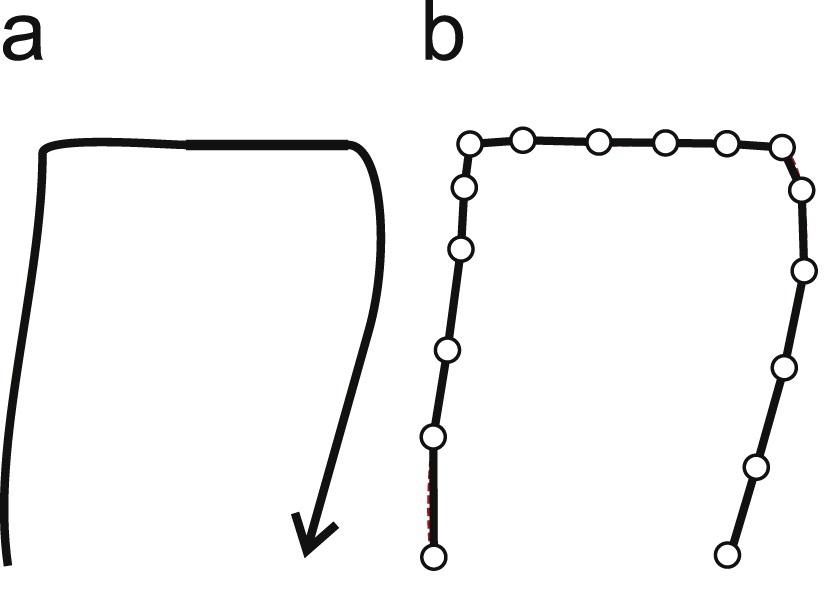
\includegraphics[width=0.7\textwidth]{stroke}
\caption{An input stroke (a) is provided to the application as (b) a sequence of point samples.}
\end{figure}

We will refer to this sampled sequence of points as a stroke. 
Strokes are stored as a list of points, objects containing coordinates from the sample space, sorted by time.
A sketch is comprised of a large number of these stroke objects.

\section{Spline Curves}

The input data represents an approximation of the stroke input from the user that is dependent on the sample resolution of the input device, and by extension the resolution of the display.
While this would work decently well assuming we are working with a static raster image, three dimensional sketching allows the user to move the camera.
Moving the camera will eventually result in poor quality sketches from the stored stroke data lacking sub-sample rate information that accurately reflects the intent of the original stroke.
Please see Figure for an example of this.
To remedy this, a mathematical representation of the curve is needed such that the "sampling rate" of the stroke is independent from the resolution of the input device.
In computer graphics, this is commonly accomplished with spline curves.

A spline is a collection of polynomial segments.
These segments can be linear, cubic, or any degree polynomial function.
Splines are a common solution for modeling smooth curves from a small number of points.
For this project, we use a Bézier curve function for the spline pieces.
A Bézier curve is a parametric curve commonly used in computer graphics to model infinitely scaling, smooth curves.
The curve is defined by control points P0, P1, ..., Pn, and is explicitly evaluated as follows:
\begin{align}
  \mathbf{B}(t) = {} &\sum_{i=0}^n {n\choose i}(1 - t)^{n - i}t^i\mathbf{P}_i \\
                = {} &(1 - t)^n\mathbf{P}_0 + {n\choose 1}(1 - t)^{n - 1}t\mathbf{P}_1 + \cdots \\
                  {} &\cdots + {n\choose n - 1}(1 - t)t^{n - 1}\mathbf{P}_{n - 1} + t^n\mathbf{P}_n,\quad 0 \le t \le 1
\end{align}
where $\scriptstyle {n \choose i}$ are the binomial coefficients, defined as
\begin{equation}
\binom nk = \binom{n-1}{k-1} + \binom{n-1}k \quad \text{for all integers }n,k : 1\le k\le n-1
\end{equation}
with initial values 
\begin{equation}
\binom n0 = \binom nn = 1 \quad \text{for all integers } n\ge0
\end{equation}
The curve can also be evaluated recursively, by
\begin{align}
\mathbf{B}_{\mathbf{P}_0}(t) = \mathbf{P}_0 \\
\mathbf{B}(t) = \mathbf{B}_{\mathbf{P}_0\mathbf{P}_1\ldots\mathbf{P}_n}(t) = (1-t)\mathbf{B}_{\mathbf{P}_0\mathbf{P}_1\ldots\mathbf{P}_{n-1}}(t) + t\mathbf{B}_{\mathbf{P}_1\mathbf{P}_2\ldots\mathbf{P}_n}(t)
\end{align}
What this equation means is that a Bezier spline of order $n$ can be defined by linear interpolation between two splines of order $n - 1$.
For this project, we will use a cubic Bézier function for the spline segments.

We must now determine a method for going from our sample data to a spline curve.
A naive approach would be to generate a spline curve that passes through the all of our control points in the order they were generated.
Any series of any four distinct points can easily be converted to a cubic Bézier curve that goes through all four points in order.
While this method guarantees that the generated curve passes through all of the input control points, it is not guaranteed to generate a curve that represents the intent of the original stroke.

\begin{center}
\begin{figure}
\begin{center}
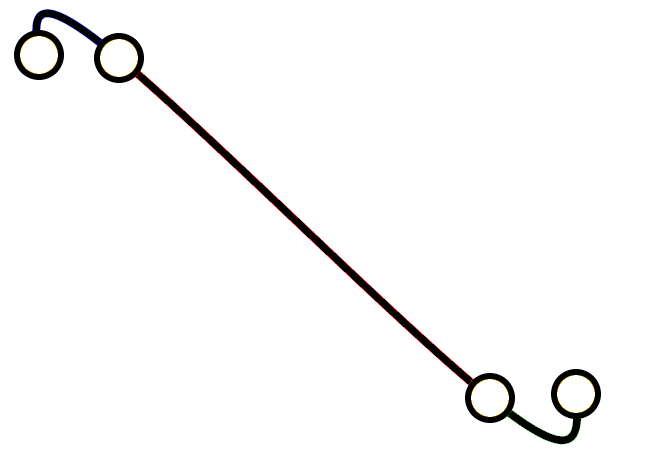
\includegraphics[width=0.8\textwidth]{splineartifact}
\end{center}
\caption{An example of an artifact in the spline generation caused by oddly spaced sample points.}
\label{fig:splineartifact}
\end{figure}
\begin{figure}
\begin{center}
\includegraphics[width=0.9\textwidth]{terminationbspline}
\end{center}
\caption{Using the distance from the control points for termination.}
\end{figure}
\end{center}

The approach we take is using the input samples as control points to generate a piecewise spline curve. 
This method is better at dealing with extreme changes in sample rates because the produced curve contains less convex and concave changes. However, it is likely that the produced curve will still be inaccurate.
The curve generated will also not pass through the sampled points. 
However, if the sample rate is high, it will be close.

In practice, not generating a curve that is exactly the same as the input sample points is not as necessary as one would think. 
The most important part is the curve should match the form of the original curve.
If the detail of the curve is important, then the user will probably draw more slowly, allowing for a greater number of sample points, and generating a spline that closely resembles the shape of the detailed section.
Also, matching control points perfectly is a poor decision when working with pixel grids, as extremely detailed sampling produces input in a staircase pattern.
Matching input exactly would make diagonal straight lines impossible.
The simpler and more consistent shape of the recursive B-spline curve makes it a better choice than the inverse control point calculation, as seen in practice by a large number of applications implementing spline approximations, including Mischief.

\subsection{Algorithm}

We begin with a list of control points, numbered from 0 to N-1. 
Segment i of the curve is influenced by control points i-1, i, i+1, and i+2.
Using this definition we can generate N-3 segments from the N control points without falling off the ends of the sequence.

Since we can't render a spline, we need to approximate the curve by subdividing it into small line segments.
We're going to divide each Bezier curve into a set of connected linear components, with the intent that a large enough number will look sufficiently smooth.
Subdivision of these segments occurs as follows:
\begin{enumerate}
\item Begin with points $\{P_0,P_1,P_2,P_3\}$, which define a Bézier curve, and a number $u, 0 \le u \le 1$
\item Define $L_1=(P_0 + P_1)*u$, $H=(P_1 + P_2)*u$, and $R_2=(P_2 + P_3)*u$
\item Define $L_2=(L_1 + H)*u$, and $R_1=(H + R_2)*u$
\item Define $M=(L_2 + R_1)*u$
\item Create two new Bézier curves using $\{P_0,L_1,L_2,M\}$ and $\{M,R_1,R_2,P_3\}$
\item Repeat steps 2 through 5 until a termination criteria is met. Possible criteria include distance between control points, and distance between control points $P_1$ and $P_2$ and the line between $P_0$ and $P_3$.
\end{enumerate}
If the termination criteria is small enough, then the curve will appear very smooth, even when zooming in to the curve.
This algorithm produces a smooth B-spline curve starting at control point 0 and ending at N-1.

\section{Summary}
In this section, we described how we turn user input over a set of pixel coordinates into a curve approximating the intent of the stroke.
We believe intent is more important than perfect accuracy since in practice, replicating curves that perfectly match input data results in poor quality curves.
This is because of the finite resolution of a pixel grid, where as in real world sketching, the concept of 'input resolution' does not exist.
Using a B-spline algorithm with cubic Bezier components, we can calculate a smooth spline curve for our stroke input.